In our benchmarks, we are concerned with measuring the growth of certain 
metrics when the number of clauses in the disjunction increases. Suppose 
we have a disjunctive zero-knowledge proof $\Pi = (A, Z, \phi)$, then 
the metrics we are concerned with are as follows:
\begin{enumerate}
  \item \textbf{Communication Complexity:} 
  size of communication between the prover and verifier (in bytes). This is 
  the size of the messages $a \leftarrow A$, $z \leftarrow Z$, and $c \leftarrow \{0,1\}^\kappa$.
  \item \textbf{Prover Computation Time:}
  time taken for the prover to run the algorithms $A$ and $Z$ 
  \item \textbf{Verifier Computation Time:}
  time taken for the verifier to run the algorithm $\phi$.
\end{enumerate}

Crucially, we are also interested in learning the \textbf{total computational time} of 
the compiled proof, which we can be easily computed by summing the prover and verifier 
running times. 

We target these three metrics as they are the main properties 
that are measurable and are used for evaluating the performance of the compiled 
proofs. Other properties such as security limitations (e.g. the requirement for a
trusted setup) are not measurable and thus are not considered in our benchmarks.

The range we use for our clauses is $(2, 2^2, \ldots, 2^{13})$; this means that 
at each step, we double the number of clauses until we reach $2^{13} = 8192$ clauses. 
Theoretically, the maximum number of clauses our compilers can accept is much larger than 
this\footnote{The limit for CDS94 is $2^{252}$ (constrained by the size of the Ristretto group 
\cite{ristretto_web} that we use for Shamir's secret sharing), and for Stacking Sigmas the number 
is theoretically unbounded.}, however, the proofs take too long to run after a certain number of clauses. 
After consulting the project supervisor, we decided that this is a suitable range for our benchmarks, 
as it allows us to measure a large range while ensuring benchmarks keep to a reasonable running time. 

\subsection{Benchmarking Tools}
Next, we discuss the choice of tools we use to construct and 
analyse our benchmarks.

\paragraph{Criterion.} We use the \texttt{criterion} library \cite{criterion} to construct our 
benchmark tests. Compared to the standard benchmarking library provided by the Rust language \cite{cargo-bench},
\texttt{criterion} is a statistics-driven benchmarking library that provides a simple API for writing benchmarks, 
automatically providing the mean, standard deviation, and the confidence interval for each benchmark. 
It also includes useful defaults such as the number of samples to run for each benchmark, a standard 
warmup time before collecting, and an HTML report generator. We provide examples of 
the HTML report generated automatically by \texttt{criterion} in Figure 
\ref{fig:criterion-report} below. 
Naturally, after some initial research, we made the decision to use \texttt{criterion}
due to the abundance of useful features and applicability to our project. 

\paragraph{Helper Interfaces.} In our design, we also decided 
to include a \texttt{Message} interface that aids in the measurement of the 
communication size of each benchmark. This interface is inspired by one of 
the same name in Hall-Andersen's implementation \cite{MHAStackSig}. 

This interface requires that the type implement a few methods that are ultimately
used to measure the size of the messages sent between the prover and verifier. 
By implementing this interface, future developers can easily measure the size 
of these messages within benchmarks with a single call to the \texttt{size()} method. 
Furthermore, we improved on the interface by requiring that it "inherit" another interface, 
\texttt{Default}, which asserts that a method is written for constructing
a default instance of the type that implements \texttt{Message}. This provides 
further utility when writing tests and benchmarks, and helps to improve the 
overall usability of the compiler.

\paragraph{Data Analysis.} To analyse our data, we collect the mean 
of each benchmark provided by \texttt{criterion} \cite{criterion} and save it in a 
CSV (comma-separated values) file. We then employ the use of Python data analysis libraries 
\texttt{pandas} \cite{reback2020pandas,mckinney-proc-scipy-2010} 
and \texttt{plotly} \cite{plotly} to parse and plot the data 
respectively. We chose these two libraries as they are widely used in data science, 
and have the necessary functions we need to parse data and produce high-quality plots.

\begin{figure}
  \centering
  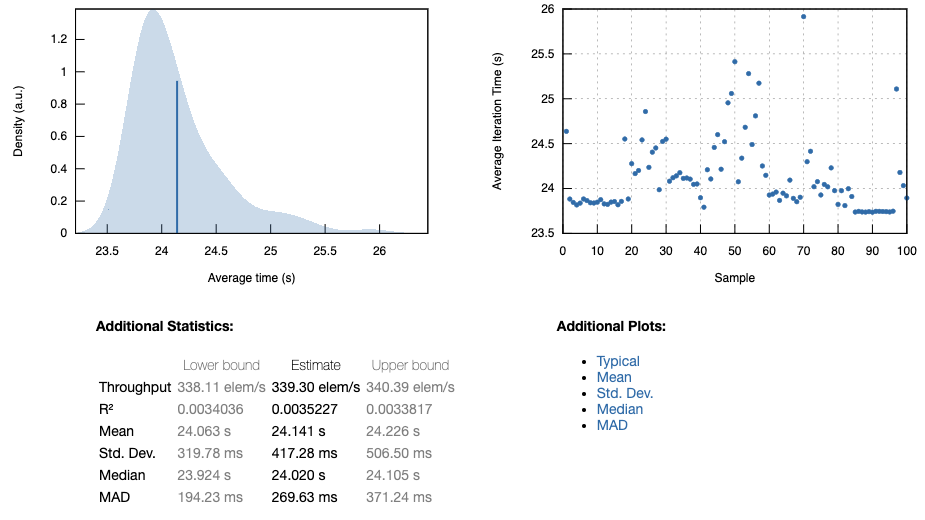
\includegraphics[width=0.9\linewidth]{../assets/html-report-example.png}
  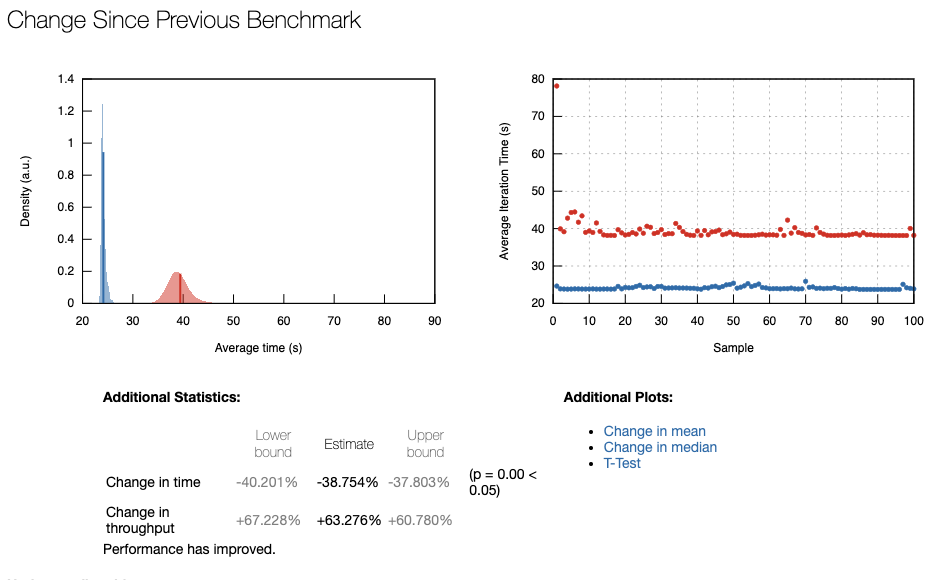
\includegraphics[width=0.9\linewidth]{../assets/performance-change-examplel.png}
  \caption{Example of the HTML report generated by \texttt{criterion}.
  The first image shows an example of the additional statistics that are 
  conveniently provided in the report. The second image shows an example of 
  the performance comparison between two different benchmark runs. If the 
  change in performance falls within a certain threshold, the change is marked as 
  significant.
  }
  \label{fig:criterion-report}
\end{figure}

\subsection{Implementation of Benchmarks}
\label{sec:benchmarks-implementation}
Our goal is to measure the metrics shared earlier and to visualise the data on 
a plot. The main challenge in this task is to ensure that the benchmarks are 
accurate and reliable -- only necessary computation should be measured, and 
appropriate calculations should be used to measure communication size. Hence, 
tests are not suitable for evaluating the validity of our benchmarks and 
will require a more manual process of accessing the data and ensuring that
the benchmarks are appropriate. In the following subsections, we discuss how 
we implement our benchmarks to achieve these goals. 

\subsubsection{Computation Time} Recall the definition of a $\Sigma$-protocol 
$\Pi = (A, Z, \phi)$. To ensure that we are measuring an accurate estimate 
of the computation time of the prover and verifier, we design and implement the 
benchmarks such that they isolate the execution of the prover algorithms ($A$ and $Z$), 
and the verifier algorithms ($\phi$ and $c \leftarrow \{0,1\}^\kappa$). The key idea 
is that we are implementing a benchmark, hence there is no need to run the 
$\Sigma$-protocol in 
order. We simply precompute the challenge $c$ from the second round of the protocol 
without measuring the time taken to compute it. Next, we execute algorithms $A$ and $Z$ 
in the prover's benchmark, collecting 
data on the computation time. Within this benchmark, 
there may be additional executions that we are not directly interested in but are 
necessary. 
Here we provide an example from the benchmarks of CDS94:


\begin{lstlisting}[language=rust]
  // Precompute challenge
  let challenge = Scalar::random(&mut verifier_rng);

  // Initialize variables to store results from the first and third round 
  let mut message_a: Vec<CompressedRistretto> =
      Vec::new();
  let mut message_z: Vec<(usize, Scalar, Scalar)> =
      Vec::new();

  // Benchmarking environment for Prover benchmark
  group.bench_with_input(
      BenchmarkId::new("prover_bench", &proverparams),
      &mut proverparams,
      |b, s| {
          b.iter(|| {
              // Code within these braces is being benchmarked and measured
              // Should have negligible cost 
              let prover_rng = &mut s
                  .prover_rng
                  .clone();
              // First round of protocol
              let (transcripts, commitments) =
                  SelfCompiler94::first(
                      &s.statement,
                      &s.witness,
                      prover_rng,
                  );
              // Third round of protocol
              let proof = SelfCompiler94::third(
                  &s.statement,
                  transcripts,
                  &s.witness,
                  &s.challenge,
                  prover_rng,
              );
              // Should have negligible cost
              message_a = commitments;
              message_z = proof;
          })
      },
  );

  /// ...

  let verifier_rng = &mut ChaCha20Rng::from_entropy();

  // Benchmarking environment for Verifier benchmark
  group.bench_with_input(
      BenchmarkId::new("verifier_bench", &v_params),
      &v_params,
      |b, s| {
          b.iter(|| {
              // Re-execution of second round
              SelfCompiler94::<Schnorr>::second(
                  verifier_rng,
              );
              // Verification algorithm
              SelfCompiler94::verify(
                  &s.statement,
                  &s.message_a,
                  &s.challenge,
                  &s.message_z,
              )
          })
      },
  );
\end{lstlisting}

On lines 17 and 36 of the code listing, we indicate (with comments) the blocks 
of code that are necessary and should have negligible cost. These are needed 
to ensure the protocol executes without error and that the output from the 
first and third rounds can be collected for the verifier's benchmark. Within the 
verifier's benchmark, we re-execute the second round of the protocol (line 53) to ensure
that the verifier's computation time for this round is also measured even though 
the resulting challenge is not used in the verification algorithm.

\subsubsection{Communication Size} 
As mentioned earlier, we use the \texttt{Message} interface to conveniently 
compute the communication size of each benchmark. Once the interface is 
implemented for each required type, measuring the size of the messages 
can be done with a single call to the \texttt{size()} method. 

\begin{lstlisting}[language=rust]
  let mut communication_sizes: Vec<usize> =
        Vec::with_capacity(Q - 1);

  /// ...

  communication_sizes.push(
      message_a.size()
          + message_z.size()
          + challenge.size(),
  );
\end{lstlisting}

To calculate the total communication size, we simply sum the sizes of the 
messages from each round of the protocol. We append this to a vector of 
communication sizes for each number of benchmarks and use this to 
plot the growth of communication size against the number of clauses. 